\documentclass[8pt]{beamer}
\usepackage[utf8]{inputenc}
\usepackage{ulem}
\usepackage{xcolor}
\usepackage{colortbl}
\usepackage{epsfig}
% \usepackage{cancel}
\usepackage{ulem}
% \usepackage{threeparttable} % Joao Pela: 
\usepackage{amsmath}
\usepackage{hyperref}
\usepackage{appendixnumberbeamer}
\usepackage{pdfpages}
\usepackage{listings}
\usepackage{animate}
% \usepackage{feynmp}         % For latex produced Feynman Diagrams

% Rule for feynmp diagrams to be considered graphics
% \DeclareGraphicsRule{*}{mps}{*}{}
% 
% % New compile sequence for feynmp
% \makeatletter
% \def\endfmffile{%
%   \fmfcmd{\p@rcent\space the end.^^J%
%           end.^^J%
%           endinput;}%
%   \if@fmfio
%     \immediate\closeout\@outfmf
%   \fi
%   \ifnum\pdfshellescape=\@ne
%     \immediate\write18{mpost \thefmffile}%
%   \fi}
% \makeatother

\lstset{language=C++,
  backgroundcolor=\color{white}, 
  basicstyle=\tiny\ttfamily,
  keywordstyle=\color{blue}\tiny\ttfamily,
  stringstyle=\color{red}\tiny\ttfamily,
  commentstyle=\color{green}\tiny\ttfamily,
  showspaces=false,
  showstringspaces=false,
  morecomment=[l][\color{magenta}]{\#}
}

\usetheme{Madrid}

\author[J. Pela]{J. Pela}
\title{Multithreading with C++ and the BOOST library}
\institute[ICL]{Imperial College London}
\date{2014-07-22}

% The log drawn in the upper right corner.
\logo{\includegraphics[height=0.115\paperheight]{img/Logo_CMSICL.png}}

\begin{document}
\setlength{\unitlength}{1mm}

% ###################################################
\begin{frame}
  \titlepage
\end{frame}

% ###################################################
\begin{frame}{Disclaimer}

\begin{block}{About me...}
 
\begin{itemize}
  \item I am not an expert in multi-threading... 
  \item I am a user with some experience and understanding of this subject and I will share that with you.
\end{itemize}

\end{block}

\begin{block}{About this presentation...}
 
\begin{itemize}
  \item This is not a complete guide on the subject of multiple threads... it offers one possible approach.
  \item Many things I will show are reflection my understanding of this subject and should not be understood as such :)
\end{itemize}

\end{block}

\begin{block}{About the usage}
 
\begin{itemize}
  \item Multithreading is very useful but may be restricted in some environments, like the IC batch system, so always think before you code and don't annoy system admins. ;)
\end{itemize}

\end{block}

\end{frame}

% ###################################################
\begin{frame}{What is multithreading?}

Multithreading is a widespread programming and execution model that:

\begin{columns}
 
\column[t]{0.50\linewidth}
\begin{block}{Definition:}
 
\begin{itemize}
  \item Allows multiple threads to exist within the context of a single process.
  \item Threads share the process's resources, but are able to execute independently.
  \item Provides developers with a useful abstraction of concurrent execution.
  \item Can also be applied to a single process to enable parallel execution on a multiprocessing system.
\end{itemize}
 
\end{block}
\column[t]{0.40\linewidth}
 
\begin{block}

\includegraphics[width=\linewidth]{img/Suffolk_Downs_horse_racing.JPG}

\end{block}

\end{columns}

\end{frame}

% ###################################################
\begin{frame}{Evoluting of computing}
 
In the last year we have seen a tendency for single core performance to stabilise and the number of cores to increase in the CPU market. 

\begin{columns}

\column[t]{0.50\linewidth}
\begin{block}{Evolution of CPU performance}
 
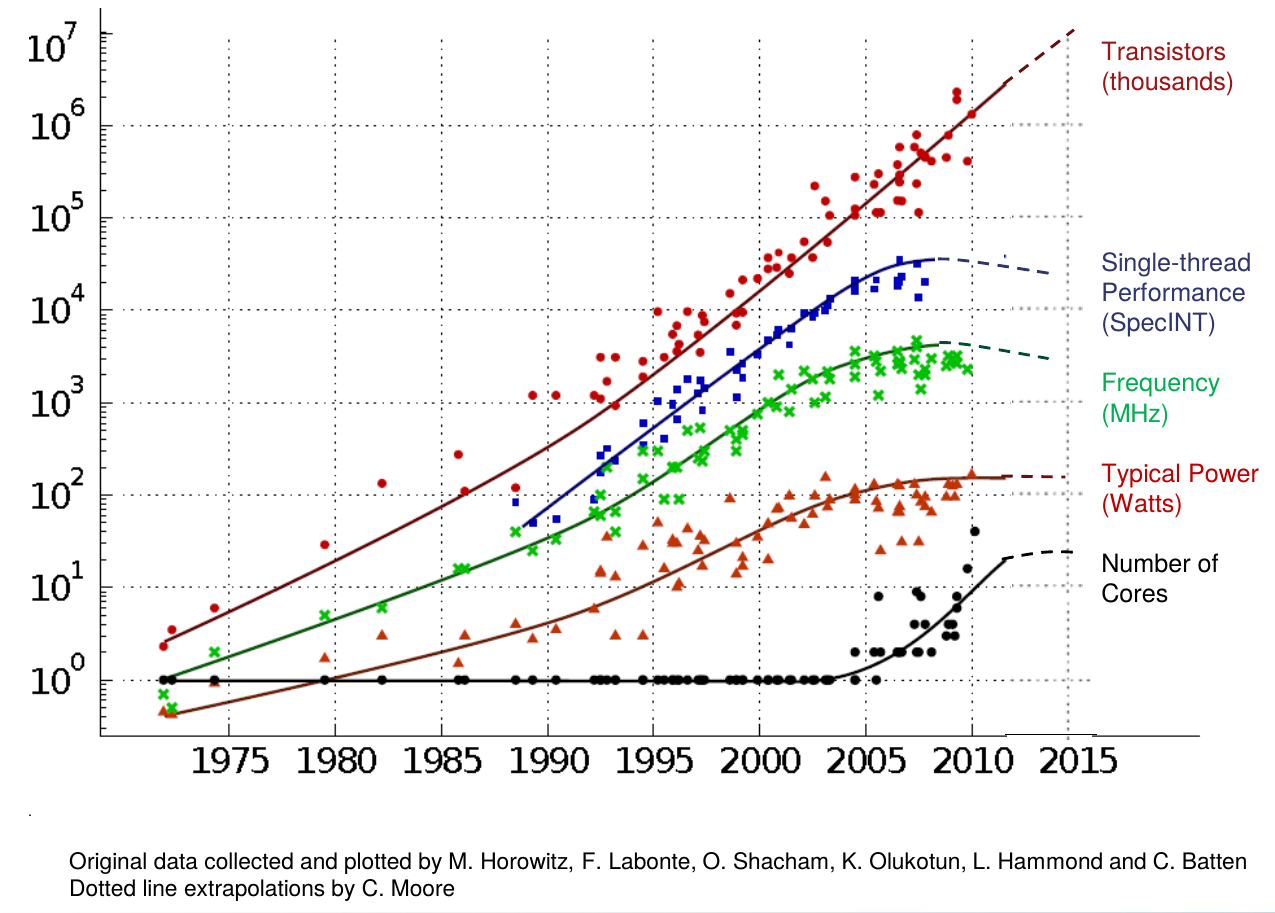
\includegraphics[width=\linewidth]{img/EvolutionOfTheCPU.png}
 
\end{block}

\column[t]{0.40\linewidth}
\begin{block}{Reasons}

\begin{itemize}
  \item Reaching the minimum size limit for a single transistor
  \item Difficulty in increasing clock speed
  \item Increasing complexity of each CPU core: optimisation, additional instructions, etc.
\end{itemize}
 
\end{block}

\begin{block}{Solution}

Make CPUs with lots cores working in parallel. But this implies code that can run in multiple execution threads!

\end{block}

\end{columns}

\begin{center}
Obviously there are several advantages and disadvantages in this approach! Lets look at some:
\end{center}
 
\end{frame}


% ###################################################
\begin{frame}{Multithreading: Advantages and disadvantages.}
 
\begin{block}{Advantages:}

\begin{itemize}
  \item Theoretically optimal multithreaded code can be the number of available cores times faster that any single core code.
  \item Allows better resource usage since several processors will use the same resources thus less resources will be idle.
  \item Can split low speed operations (example: file access from disk) from high speed calculations thus removing idle unnecessary idle times.
  \item In low power applications allow to switch off completely some of the cores allowing to only have minimal necessary resources powered.
  \item GPUs take this approach even further and some boards out there have +1000 cores.
\end{itemize}

\end{block}

\begin{block}{Disadvantages.}
 
\begin{itemize}
  \item Dealing with multiple threads opens several new classes of problems in coding which can be very hard to debug.
  \item Sharing resources may also create overheads at hardware and software level.
  \item Greater exposure of the hardware to OS and user programs thus increasing complexity of code.
\end{itemize}
 
\end{block}

\begin{center}
This are just some of the issues to consider.  
\end{center}

\end{frame}

% ###################################################
\begin{frame}{Why BOOST?}
 
\begin{block}{BOOST Library}

BOOST is an extensive C++ library that:

\begin{itemize}
  \item Widely used available over multiple platforms in a portable way 
  \item Covers multiple topics: date/time manipulation, filesystem interfaces, networking, numerical programming, interprocess communication, etc.
  \item Good documentation with lots of examples.
  \item Well maintained with frequent updates and bug fixes. 
\end{itemize}

\end{block}

\begin{block}{BOOST Multithreading}
 
\begin{itemize}
  \item Provides complete support to thread handling.
  \item Package classes are portable thus allowing OS independent code.
  \item Many examples and good community support. 
\end{itemize}
 
\end{block}
 
\end{frame}

% ###################################################
\begin{frame}[fragile]{BOOST Threads}
\footnotesize
 
\begin{block}{The class \uline{boost::thread}}
\footnotesize

\begin{itemize}
  \item Is the representation on the boost library of a single thread of execution. 
  \item This interface is implemented in the platforms where boost is available allowing making portable multithreaded code.
  \item Normally boost::thread object is constructed by passing the function or method it is to be run.
\end{itemize}

NOTE: A thread object can be set to a special state of not-a-thread, in which case it is inactive

\end{block}

\begin{exampleblock}{Compiling examples on this tutorial}

For your system you need to supply boost headers and libraries location. For my system (opensuse linux) would be:

\begin{lstlisting}
g++ <input_file>.cxx -o <output_file>.exe -I/usr/include/boost -L/usr/lib64 -lboost_thread-mt -lboost_system
\end{lstlisting}
\end{exampleblock}

\begin{exampleblock}{Simulating work}

To simulate real work we are going to simple use boost "wait" function :D

\begin{lstlisting}
boost::posix_time::seconds workTime(3);
boost::this_thread::sleep(workTime);
\end{lstlisting}

Note that \uline{boost::this\_thread} gives us a convenient refer to the currently running thread.

\end{exampleblock}
 
\end{frame}

% ###################################################
\begin{frame}[fragile]{Type A: A Thread Function}
 
\begin{columns}
 
\column[t]{0.45\linewidth}
\begin{exampleblock}{Example A}

\begin{lstlisting}
#include <iostream>
#include <boost/thread.hpp>
#include <boost/date_time.hpp>

using namespace std;

void workerFunc(){

    boost::posix_time::seconds workTime(3);
    cout << "Worker: running" << endl;

    // Pretend to do something useful...
    boost::this_thread::sleep(workTime);
    cout << "Worker: finished" << endl;
}

int main(int argc, char* argv[]){

    cout << "main: startup" << endl;
    boost::thread workerThread(workerFunc);

    cout << "main: waiting for thread" << endl;
    workerThread.join();
    cout << "main: done" << endl;

    return 0;
}
\end{lstlisting}

\end{exampleblock}
 
\column[t]{0.50\linewidth}
\begin{block}{What is happening?}

Here we just pass a basic C-style function to \uline{boost::thread} constructor.
\begin{itemize}
  \item The function will start running immediately.
  \item We can wait (in the main thread) for the threaded function to complete by calling \uline{join()}.
\end{itemize}

\end{block}
\begin{block}{Diagram:}
\centering

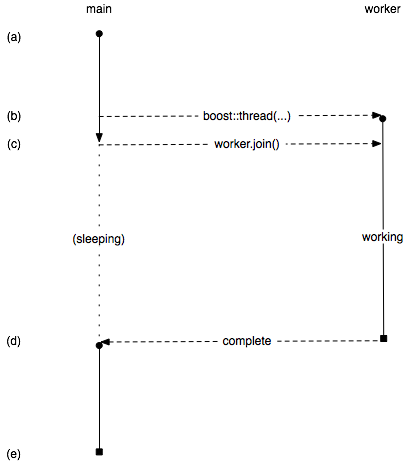
\includegraphics[width=0.45\linewidth]{img/BoostThreadExample.png}
 
\end{block}

\end{columns}
 
\end{frame}

% ###################################################
\begin{frame}[fragile]{Type A: Passing Arguments}

This last example not not very useful, we probably would like to pass some parameters to out function for processing. Let;s do that:

\begin{itemize}
  \item simply add parameters to the thread object’s constructor
  \item arguments will automatically be and passed in to the thread function
\end{itemize}

\begin{exampleblock}{Contructor}

\begin{lstlisting}
void workerFunc(const char* msg, unsigned delaySecs) //...
\end{lstlisting}

\end{exampleblock}

Now pass the arguments to the thread constructor after the name of the thread function:

\begin{exampleblock}{Creating the thread}

\begin{lstlisting}
boost::thread workerThread(workerFunc, "Hello, boost!", 3);
\end{lstlisting}

\end{exampleblock}

\begin{block}{Exercise:}

It's your turn now! Let's try to implement, compile and run this example! (5 min)
 
\end{block}

\end{frame}

% ###################################################
\begin{frame}[fragile]{Type B: Functor}
 
\vspace{-15px}
\begin{columns}
 
\column[t]{0.55\linewidth}
\begin{exampleblock}{Functor}

\begin{lstlisting}
class Worker{
public:
  Worker(unsigned delaySecs) : m_delay(delaySecs){}

  void operator()(){
    boost::posix_time::seconds workTime(m_delay);
    std::cout << "Worker: running" << std::endl;
  
    boost::this_thread::sleep(workTime);
    std::cout << "Worker: finished" << std::endl;
  }
    
private:
  unsigned m_delay;
};
\end{lstlisting}

\end{exampleblock}
\vspace{-8px} 
\begin{exampleblock}{Main program:}

\begin{lstlisting}
int main(int argc, char* argv[]){

    std::cout << "main: startup" << std::endl;
    Worker w(3);
    boost::thread workerThread(w);

    std::cout << "main: waiting for thread" << std::endl;
    workerThread.join();
    std::cout << "main: done" << std::endl;

    return 0;
}
\end{lstlisting}

\end{exampleblock}
 
\column[t]{0.40\linewidth}

\begin{block}{Functor}

Functor is a name of an object that can be called like a function.

\begin{itemize}
  \item The class defines a special method by overloading the operator() 
  \item This operator will be invoked when the functor is called
  \item This allows the functor to encapsulate the thread’s context and still behave like a thread function.
\end{itemize}

\end{block}
\vspace{-8px}
\begin{block}{Main code}
 
\begin{itemize}
  \item We create our callable object with all necessary parameters.
  \item Pass the instance to the boost::thread constructor, which will invoke the operator()()
  \item This becomes a new thread and as access to all objects context and methods.
\end{itemize}

\end{block}

\end{columns}
 
\end{frame}

% ###################################################
\begin{frame}[fragile]{Type C: Method in a thread}

Sometimes its convenient to define an object with an instance method that runs on its own thread. This can be done easily with BOOST.

\begin{block}{What to do?}

\begin{itemize}
  \item We will be making a regular function into a thread.
  \item We have to pass the method address to boost thread via the class qualifier.
  \item On C++ all methods receive a implicit "this" as first parameter, we need to replicate that behavior.
  \item then we will pass the remaining parameters.
\end{itemize}

\end{block}

\begin{exampleblock}{Code:}

\begin{lstlisting}
Worker w(3);
boost::thread workerThread(&Worker::processQueue, &w, 2);
\end{lstlisting}

\end{exampleblock}

NOTE: be careful to not destroy the object while the thread is running since this will create a, difficult to debug, mess in memory.

\end{frame}

% ###################################################
\begin{frame}[fragile]{Type D: Object encapsulated thread}

You may want to make classes that manage their own threads. Thus whole process of creation, handling and destruction of new threads is encapsulated.

\begin{columns}
  
\column[t]{0.48\linewidth}
\begin{exampleblock}{Class code}

\begin{lstlisting}
//...
void start(int N){
  m_Thread = boost::thread(&Worker::doRun,this,N);
}

void join(){
  m_Thread.join();
}

private:
  boost::thread m_Thread;
//...
\end{lstlisting}

\end{exampleblock}
 
\begin{exampleblock}{Main code}

\begin{lstlisting} 
Worker worker;
worker.start(3);
worker.join();
\end{lstlisting}

\end{exampleblock}
 
\column[t]{0.47\linewidth}

\begin{block}{Structure}
\footnotesize

\begin{itemize}
  \item The thread object will exist as an instance member (as opposed to a pointer).
  \item In this case the default constructor for the thread creates it in an invalid state called "not-a-thread".
  \item Thread instance will wait until we assing a real one to start.
\end{itemize}

\begin{itemize}
  \item Method Worker::start() spawns a thread that will run method doRun.
  \item Method Worker::join() will call the tread join().
\end{itemize}

So on the main code we do not need to have any thread action only direct interaction with the object.

\end{block}

\begin{block}{Exercise:}
\footnotesize

It's your turn now! Let's try to implement, compile and run this example! (5 min)
 
\end{block} 
 
\end{columns}

\end{frame}

% ###################################################
\begin{frame}{Topic conclusions}
 
We have seen several techniques to create and handle threads with BOOST

\begin{block}{Types of implementation:}
 
\begin{itemize}
  \item Type A: C-Style function
  \item Type B: Functor
  \item Type C: Method in a thread
  \item Type D: Object encapsulated thread
\end{itemize}
 
\end{block}

BOOST allows great flexibility and ease in implementing multithread code. But there are many possible problems to consider. Let's look at some:
 
\end{frame}

% ###################################################
\begin{frame}{Problems: shared state}

Up to now all examples that we looked had only 2 threads and had no shared state. What is meant by shared state is any shared data or resources between threads:

\begin{columns}

\column[t]{0.45\linewidth}
\begin{block}{Shared state}
 
\begin{itemize}
  \item such as file handle
  \item socket
  \item graphics context
  \item queue
  \item buffer
  \item ...
\end{itemize}
 
\end{block}

\column[t]{0.45\linewidth}
\begin{block}{If two threads are truly independent}

\begin{itemize}
  \item They can safely run concurrently without care or consideration. 
  \item We wouldn’t need sophisticated mechanisms for synchronisation.
\end{itemize}

\end{block}

\end{columns}

\begin{itemize}
  \item As soon as you introduce shared state, you have to worry about atomicity, consistency, race conditions, and all sorts of issues.
  \item So one of the first design considerations for concurrent systems is to try to minimise the amount of shared state between threads.
\end{itemize}

\end{frame}

% ###################################################
\begin{frame}{Problems: atomicity}
 
An operation is atomic if the operation completes without interruption. It is never partially complete, which may leave the system or data in an inconsistent or invalid state.

\begin{block}{Classic example: Bank transfer (pay landlord)}
\footnotesize

\begin{columns}
 
\column[t]{0.45\linewidth}
Operations:
\begin{itemize}
  \item Ensure you have sufficient funds
  \item Ensure the receiving account number is valid
  \item Withdraw the £1200 in funds from your account
  \item Deposit the £1200 in the landlord’s account
\end{itemize}

\column[t]{0.45\linewidth}
What can go wrong?
\begin{itemize}
  \item Steps 1 and 2 are precondition, if operation fails there no problem.
  \item But after step 3 you "absolutely" want step 4 to complete!
  \item Steps 3 and 4 must be performed atomically
\end{itemize}

\end{columns}

\end{block}

The same concept applies to in-memory operations that must be atomic. A for this we can use mutex (for "mutual exclusion"):
\begin{itemize}
  \item Used to serialise access to resources within a region of code that must run as an atomic operation.
  \item We would lock the mutex before the transaction, and unlock it afterwards.
\end{itemize}

\end{frame}

% ###################################################
\begin{frame}[fragile]{Problems: race conditions}
\footnotesize

A race condition is a general term for a class of problems, whereby the result of an operation is at the mercy of the timing of concurrent events:
\begin{itemize}
  \item Program becomes non-deterministic, it may not always produce the correct result!
  \item One of the most subtle and difficult to debug problems in software development.
\end{itemize}

\begin{exampleblock}{Example: Counter - 1 thread incremented}
\footnotesize

One of the most basic operations in C++ is to increment (example: $m_SequenceNumber++$;) a counter and most would assume this is an atomic action, but in fact (in x86 architecture) would be:

\begin{lstlisting} 
movl    -12(%ebp), %eax
incl    %eax
movl    %eax, -12(%ebp)
\end{lstlisting}

So even a simple operation can consist of several operation in memory (3 operations in this case load: increment, then store).

\end{exampleblock}
\footnotesize

There are two potential points that a race condition could occur: between the load and the increment, and between the increment and the save.

\begin{exampleblock}{Example: Counter - 2 thread incremented}

\begin{lstlisting} 
Thread  Instruction               m_SequenceNumber Register
A       LOAD m_SequenceNumber,R0  234              234
A       INCR R0                   234              235
B       LOAD m_SequenceNumber,R1  234              234
B       INCR R1                   234              235
B       STORE R1,m_SequenceNumber 235              235
A       STORE R0,m_SequenceNumber 235              235
\end{lstlisting}

So, instead of the sequence number being incremented twice, and being 236 as we would expect, the sequence number is only 235.

\end{exampleblock}

This problem can be avoided by using mutex and locking usage of our variable by other threads. But Mutexs can generate problems too... 

\end{frame}

% ###################################################
\begin{frame}[fragile]{Problems: deadlocks}
 
When more than one thread locks more than one mutex, there arises the potential for a condition known as a deadlock. 
\begin{itemize}
  \item One thread is holding a lock while waiting for another to become available
  \item Second thread is holding the second lock and waiting for the first lock to become available
  \item More complicated situations may arrives where several threads form a ring of holding and waiting for locks.
\end{itemize}

\begin{columns}

\column[t]{0.35\linewidth}
\begin{exampleblock}{Problematic code:}
 
\begin{lstlisting} 
void threadA(){
    while (running){
        mutexOne.lock();
        mutexTwo.lock();
        processStuff();
        mutexOne.unlock();
        mutexTwo.unlock();
    }
}
void threadB(){
    while (running){
        mutexTwo.lock();
        mutexOne.lock();
        processStuff();
        mutexTwo.unlock();
        mutexOne.unlock();
    }
}
\end{lstlisting}

\end{exampleblock}

\column[t]{0.60\linewidth}
\begin{block}{Diagram:}
\centering 
 
\animategraphics[autoplay,loop,height=2.7cm]{1}{img/DeadlockAnimation_}{0}{7} 

\end{block}

\end{columns}

The problem of deadlocks can (largely) be avoided by consistently locking mutexes in the same order, and unlocking them in reverse order.

\end{frame}

% ###################################################
\begin{frame}[fragile]{Problems: exceptions}
 
Exceptions in $C++$ can be a very effective mechanism for error handling. However, like many $C++$ features, care must be taken, especially in threads. 
\begin{itemize}
  \item A thread is destroyed when the thread function returns.
  \item Uncaught exceptions can cause the entire thread to exit, without warning or notice.
  \item So if you have a thread that mysteriously disappears, an uncaught exception is a likely culprit.
\end{itemize}

If you wish to avoid your thread being killed, you should add a top-level try-catch block.
\begin{itemize}
  \item You may simply log the uncaught exception then exit.
  \item You may resume thread processing if it is safe to do so.
\end{itemize}
 
\begin{exampleblock}{Code:}
 
\begin{lstlisting}
void processThread(){

  while(keepProcessing){
    try{// Do actual work}
        
     // Catch more specific exceptions first if you can
     catch (std::exception& exc){
       log("Uncaught exception: " + exc.what());
       // Maybe return here?
     }
  }
}
\end{lstlisting}

\end{exampleblock}

Just as an errant exception can cause havoc with threads running, they can also cause problems with mutexes. We can use lock guard to ensure mutexes are unlocked, even if an exception is thrown.
 
\end{frame}

% ###################################################
\begin{frame}{Problems: other problems}
 
There are more categories of problems you may encounter but they fall out of the scope of today's presentation. But just to reinforce the idea that multithreaded programming is not a trivial undertaking, 
I leaving you a list of some other problem categories for further studies:

\begin{itemize}
  \item starvation
  \item priority inversion
  \item high scheduling latency
  \item ...
\end{itemize}

Mutithreading is currently an active research and development area and issues such as the ones presented today should be always considered for concurrent programming. 
 
\end{frame}

% ###################################################
\begin{frame}{Topic conclusions}

Most typical problems with multi-threading are well known and there are clear solutions for them and is possible to write robust code in this paradigm but one must be careful to avoid the many pitfalls. 

\begin{block}{Somethings to take into account in your coding:}
 
\begin{itemize}
  \item Minimise shared state
  \item Program defensively
  \item Assume your threading code can be preempted at any time
  \item Identify shared resources and protect them with mutexes
  \item Identify algorithms that need to be atomic
  \item Identify code with dependent results that needs to be atomic
  \item Minimise the number of resources shared between threads
  \item Minimise the duration of locks
  \item Ensure exceptions cannot disrupt synchronisation flow
  \item Always acquire and release mutexes in the same order
\end{itemize}

\end{block}

\begin{center} 
Now lets look at the details of how to use mutexs.
\end{center}

\end{frame}

% ###################################################
\begin{frame}{Mutual exclusion:  Mutex}

\begin{block}{What is a mutex?}
 
\begin{itemize}
  \item A mutex is special kind of lock, which is used to protect shared resources.
  \item It guaranteed to be held by at most one thread at a time.
  \item Can be used as a protection mechanism for resources and data
  \item Can be used to avoid race conditions, and implement atomic operations.
\end{itemize}

\end{block}

\begin{block}{What happens if multiple threads try to lock a mutex?}

\begin{itemize}
  \item If a mutex is not locked by a thread, then any thread can potentially lock it. 
  \item If any other thread attempts to lock it, it will typically block and wait until the mutex is unlocked by the owning thread.
  \item It is also possible to return if the lock fails, or wait for a certain period of time before giving up.
\end{itemize}

\end{block}

A mutex is typically declared alongside the resource it protects. The mutex should be in the same scope as the resource, or an enclosing scope. BOOST provides 4 flavours of mutex.

\end{frame}

% ###################################################
\begin{frame}[fragile]{Type A: Regular Mutex}
 
The simplest form of mutex is a regular boost::mutex. You lock and unlock it, and only one thread can lock the mutex at a time. 

\begin{itemize}
  \item Any thread that calls lock() on a mutex held by another thread will block indefinitely (important for factor in design).
  \item This must be carefully managed to avoid program hangs.
\end{itemize}

\begin{exampleblock}{Code:}
 
\begin{lstlisting}
boost::mutex work_queue_mutex;
queue<item> work_queue;

// ...

work_queue_mutex.lock();

auto work_item = work_queue.pop();

work_queue_mutex.unlock();
\end{lstlisting}

\end{exampleblock}

Regular mutexes also have a try\_lock() method, which will return immediately with a failure status if the mutex cannot locked. 
\begin{itemize}
  \item Most threads run in a loop, so this can be useful to preform something else
  \item In the case nothing else can be done maybe putting the thread to sleep for some time may be useful
\end{itemize}
 
\end{frame}

% ###################################################
\begin{frame}[fragile]{Type B: Timed Mutexes}
 
The boost::timed\_mutex class is a subtype of boost::mutex, which adds the ability to specify a timeout. 
\begin{itemize}
  \item Attempts to lock the mutex for some time and if it cannot returns false.
  \item Takes either an absolute time, or a relative time.
\end{itemize}


\begin{exampleblock}{Code:}
 
\begin{lstlisting}
boost::mutex work_queue_mutex;
queue<item> work_queue;
TimeDuration mutex_timeout;

// ...

if (work_queue_mutex.timed_lock(mutex_timeout)){

    auto work_item = work_queue.pop();
    work_queue_mutex.unlock();
}
\end{lstlisting}

\end{exampleblock}

With some study of your application you can tune the timeout to maximise the performance of your algorithm.

\end{frame}

% ###################################################
\begin{frame}[fragile]{Type C: Recursive Mutexes}
 
Normally a mutex is locked only once, then unlocked. But on some applications may be useful to allow the same thread to lock the same mutex multiple times.
\begin{itemize}
 \item Useful for nested method calls.
 \item Situations where the thread may call multiple methods that require a given mutex lock.
 \item Still the mutex must be unlocked the same number of times that it got locked on the specific thread.
 \item This behaviour assumes that allow method the lock/unlock mutex will do so in a compartmentalised and nested way. 
\end{itemize}
 
\end{frame}

% ###################################################
\begin{frame}[fragile]{Type D: Shared Mutexes}
\footnotesize

Some concurrency scenarios involve having one writer and many readers. 
\begin{block}{Example}
\footnotesize

\begin{itemize}
 \item One thread downloading data from the network, another displaying the data on the screen and another saving the data to database.
 \item Downloading thread needs locking for writing
 \item Other two threads for reading
 \item There is no reason for the reading threads to exclude each other (concurrent reading is safe)
 \item Only when the downloading thread is writing its necessary to lock the other out.
\end{itemize}

\end{block}

\begin{columns}

\column[t]{0.40\linewidth}
\begin{exampleblock}{Code:}
 
\begin{lstlisting}
boost::mutex work_queue_mutex;
queue<item> work_queue;

// Reader thread
work_queue_mutex.read_lock();
auto work_item = work_queue.head();
work_queue_mutex.unlock();

// Writer thread
work_queue_mutex.write_lock();
auto work_item = work_queue.push(new_item);
work_queue_mutex.unlock();
\end{lstlisting}

\end{exampleblock}

\column[t]{0.55\linewidth}
\begin{block}{Summary}
\footnotesize

\begin{itemize}
  \item Any time the reading threads need to read the resource, they obtain a read-lock.
  \item Allows other read-locks to successfully access the resource, preventing a write-lock.
  \item When the writer obtains lock, readers will need to wait until update is complete.  
\end{itemize}

\end{block}

\end{columns}
 
\end{frame}

% ###################################################
\begin{frame}[fragile]{Lock/Unlock Pairing:}
 
If a mutex is not released due to a logical error (such as an uncaught exception), this is probably not recoverable. Thus it is vitally important that all lock/unlock operations appear in pairs.

To protect against this class of problem, the lock\_guard object was introduced. 
\begin{itemize}
  \item Locks the mutex for you in its constructor, and unlocks it in the destructor.
  \item If thread is destroyed for some reason the mutex is automatically released.
\end{itemize}

\begin{exampleblock}{Code:}
 
\begin{lstlisting}
unsigned applyTotals(unsigned count){

  boost::lock_guard totalsLock(mTotalsMutex);
  mTotals.globalCount += count;
  writeTotalsToDatabase();
}
\end{lstlisting}

\end{exampleblock}

The totalsLock will acquire (or wait to acquire) the mutex when created, and when it is destroyed at the end of the method, it will unlock the mutex. If an exception is thrown, the lock's destructor will still be called, and the mutex will be safely released. This ensures the operation is atomic, and can safely handle error conditions.
 
\end{frame}

% ###################################################
\begin{frame}[fragile]{Conditional variables}
 
While a mutex allows you to lock a resource for usage it tells you nothing about the content of the resource being ready for usage (example stack of events to process), this is where conditional variables can help.

\begin{exampleblock}{Code:}
 
\begin{lstlisting}
unsigned applyTotals(unsigned count){
boost::condition_variable cond;
boost::mutex mut;
bool data_ready;

void process_data();

void wait_for_data_to_process(){

  boost::unique_lock<boost::mutex> lock(mut);
  while(!data_ready){
    cond.wait(lock);
  }
  process_data();
}
\end{lstlisting}

\end{exampleblock}

Notice that the lock is passed to wait: wait will atomically add the thread to the set of threads waiting on the condition variable, and unlock the mutex. When the thread is woken, the mutex will be locked again before the call to wait returns. This allows other threads to acquire the mutex in order to update the shared data, and ensures that the data associated with the condition is correctly synchronised.
 
\end{frame}

% ###################################################
\begin{frame}{Summary and next steps}
 
\begin{block}{Today we covered}
 
\begin{itemize}
  \item Multithreading techniques using BOOST
  \item Common problems and solutions
  \item Mutex and synchronisation
  \item Conditional variables
\end{itemize}

\end{block}

\begin{block}{Thank you:}
 
\begin{itemize}
  \item Thank you for listening and I hope today's presentation helps you with your code.
  \item A good part of this presentation was based on Mr. Gavin Baker blog on C++ coding where you can find more examples.
\end{itemize}
 
\end{block}

\end{frame}

\end{document}